\section{Introduction}
The goal of this chapter is to document the observed order of accuracy and the 
grid convergence index (GCI) for various validation and verification test cases.

\subsection{Statement of the received results and their analysis}
The convergence rates for the two numerical approximation techiques used in
SWIRL will be presented for a set of test cases using MMS/MES. 


for the 
\section{Code Verificaton using the Method of Manufactured Solutions}
Figure \ref{fig:1} shows the manufactured solution for the mean flow profile. 
The tangent summation method (TSM) was used to generate the axial mach number and 
for the speed of sound.   The tangential mach number was then numerically approximated by 
using the composite trapezoidal rule. The manufactured mean flow profile 
is unique in that it has been generated solely for the verification of SWIRL 
and does not have physical significance. The ``kinks'' in the solution will allow
there to be a significant magnitude for the derivatives of these solution. 

The TSM was also used to generate the manufactured solutions for the perturbation
variables in Figures \ref{fig:1a}-\ref{fig:4a}. The boundary condition values of 
the MS for $\bar{v}_r$ $dP/dr$ must reflect the actual boundary conditions in SWIRL. 
This is set by using a fairing function. Note that the hard wall condition requires
$\bar{v}_r$ to be zero which is shown in Figure \ref{fig:1a}. While the boundaries for the 
pressure perturbation may not be known, the boundary condition is set with the 
derivative of the pressure perturbation, which may or may not be zero depending
if there is liner for the test case. This is why these functions no longer resemble
tangent function, but in essence still are. 

The results from the numerical integration is presented in Figure \ref{fig:5}. Although 
the slope of the line appears linear, the TSM was still used to generate the 
MS for the speed of sound. To demonstrate the effect of using denser grids, the 
difference between the expected speed of sound to the actual speed of sound is 
shown in Figure \ref{fig:5a} as a function of radius (needs label). 
Note that the error does not reach machine precision for the first grid and 
approaches zero as more grid points are used. 

As the error decreases, it will decrease at a known rate depending on the numerical
integration scheme used. Since the composite trapezoidal rule has an order of accuracy of 2, 
it is expected that the approximated order of accuracy will approach two as
the error approaches zero. This behavior is shown in Figure \ref{fig:8} where the approximated
line is the $L2_{norm}$ of the speed of sound error 
 The slope ( i.e. the asymptotic rate of convergence )approached two for 
 numerical integration as the grid spacing decreases (See Figure \ref{fig:9}) .

For the LEE, a second and fourth order central differencing scheme is used
for the approximated radial derivatives and then compared to the source terms 
generated for the MMS in Figure \ref{fig:6}. (Discuss Error here\dots skeptical 
on the plot\dots \ref{fig:7})

The $L2_{norm}$ and the  asymptotic rate of convergence is shown for the 
two diffferencing schemes in  \ref{fig:9} and \ref{fig:10}. (How should is dicuss this?) 


\begin{figure}[!]
    \centering
    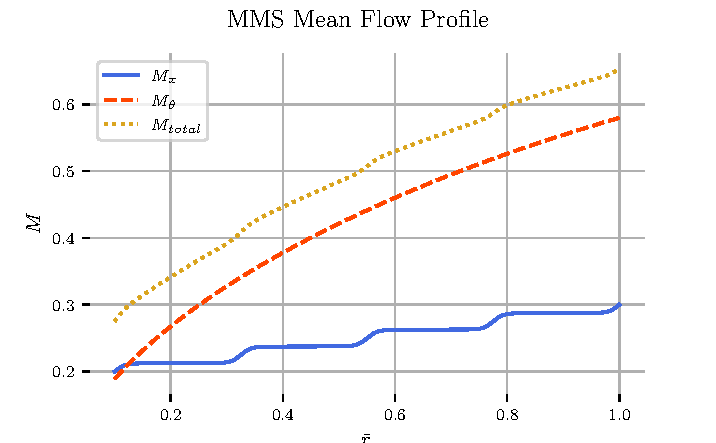
\includegraphics{/home/jeff-severino/SWIRL/CodeRun/04-plotReport/tex-outputs/MMS_mean_flow_profile.pdf}
    \caption{The manufactured mean flow test case using a summation of Tangents for $A$ and $M_x$}
    \label{fig:1}
\end{figure}


\begin{figure}[!]
    \centering
    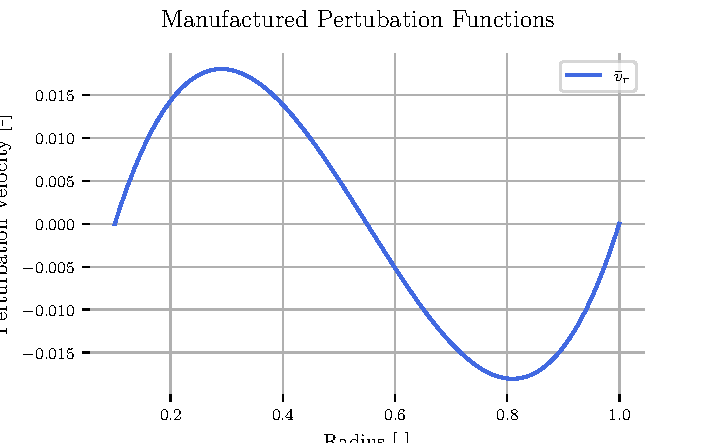
\includegraphics{/home/jeff-severino/SWIRL/CodeRun/04-plotReport/tex-outputs/MMS_perturbation_variables_vR.pdf}
\caption{The manufactured perturbation functions ,$v_r$}%, $v_x$, $v_{\theta}$, $p$}
    \label{fig:1a}
\end{figure}


\begin{figure}[!]
    \centering
    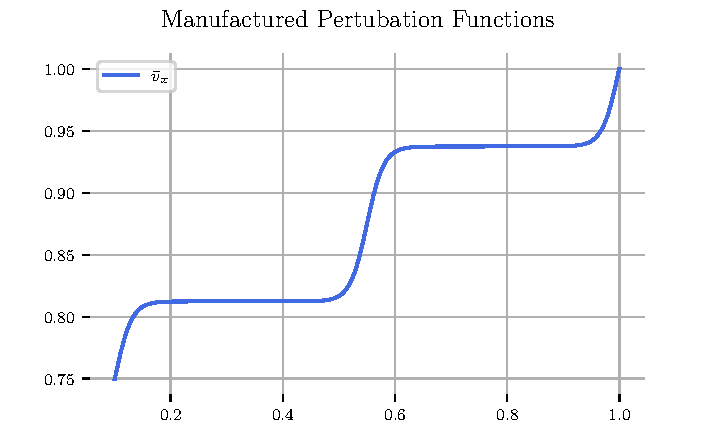
\includegraphics{/home/jeff-severino/SWIRL/CodeRun/04-plotReport/tex-outputs/MMS_perturbation_variables_vX.pdf}
\caption{The manufactured perturbation functions ,$v_x$}%, $v_x$, $v_{\theta}$, $p$}
    \label{fig:2a}
\end{figure}


\begin{figure}[!]
    \centering
    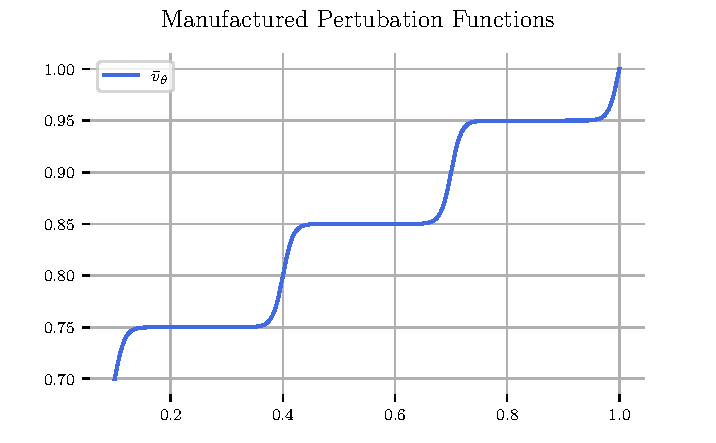
\includegraphics{/home/jeff-severino/SWIRL/CodeRun/04-plotReport/tex-outputs/MMS_perturbation_variables_vTh.pdf}
    \caption{The manufactured perturbation functions ,$v_{\theta}$}%, $v_x$, $v_{\theta}$, $p$}
    \label{fig:3a}
\end{figure}


\begin{figure}[!]
    \centering
    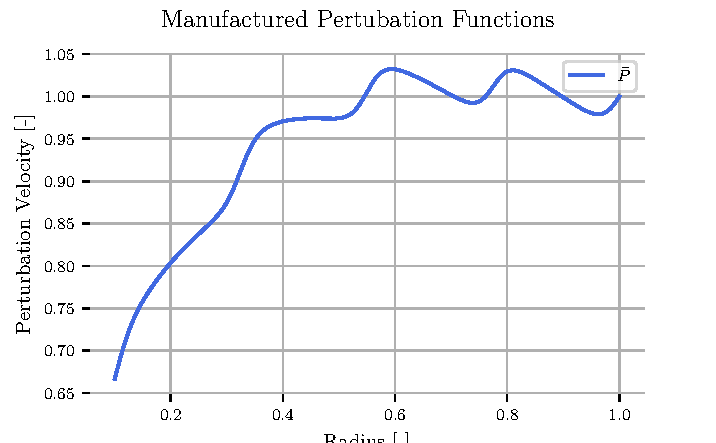
\includegraphics{/home/jeff-severino/SWIRL/CodeRun/04-plotReport/tex-outputs/MMS_perturbation_variables_Pr.pdf}
\caption{The manufactured perturbation functions ,$P$}%, $v_x$, $v_{\theta}$, $p$}
    \label{fig:4a}
\end{figure}

\begin{figure}[!]
    \centering
    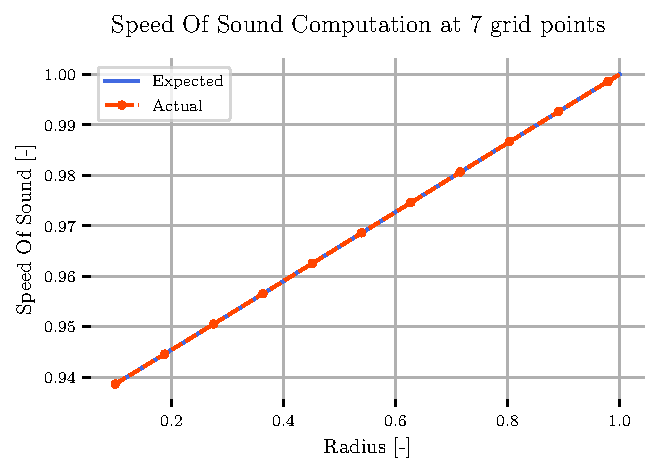
\includegraphics{/home/jeff-severino/SWIRL/CodeRun/04-plotReport/tex-outputs/SpeedOfSoundComparison1.pdf}
    \caption{ A comparison of the speed of sound, expected vs actual at the lowest grid to show similarities in solution}
    \label{fig:5}
\end{figure}


\begin{figure}[!]
    \centering
    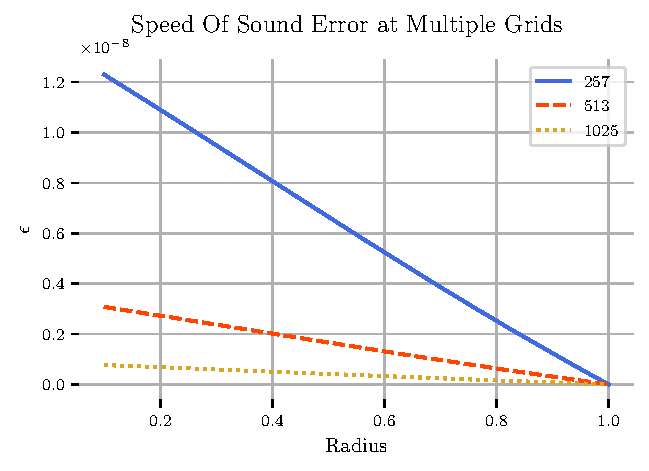
\includegraphics{/home/jeff-severino/SWIRL/CodeRun/04-plotReport/tex-outputs/SpeedOfSoundComparison2.pdf}
    \caption{ A comparison of the speed of sound error at three grid}
    \label{fig:5a}
\end{figure}


\begin{figure}[!]
    \centering
    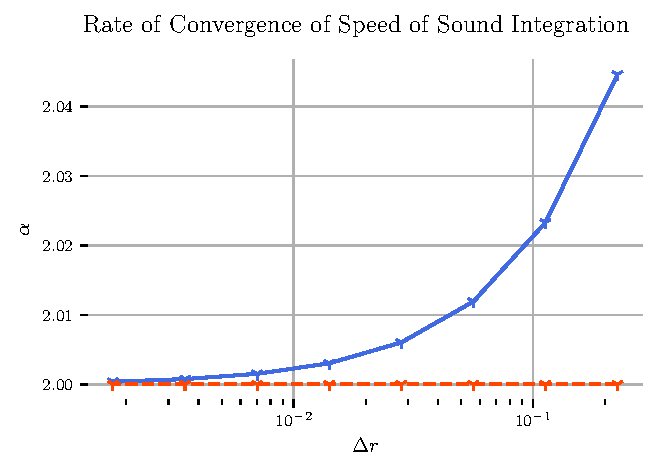
\includegraphics{/home/jeff-severino/SWIRL/CodeRun/04-plotReport/tex-outputs/SND_ROC.pdf}
    \caption{ A comparison of the speed of sound error at three grid}
    \label{fig:5a}
\end{figure}



\begin{figure}[!]
    \centering
    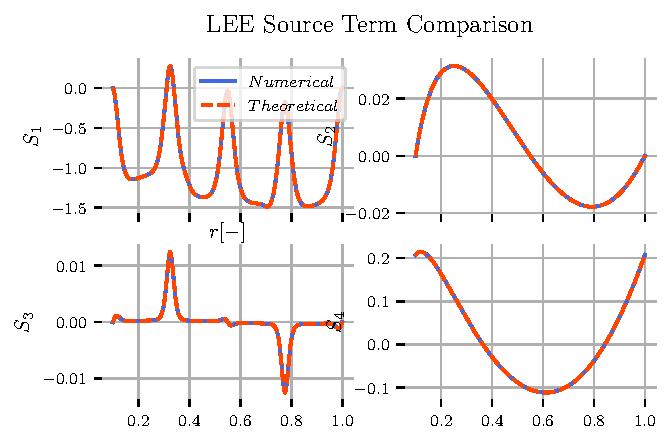
\includegraphics{/home/jeff-severino/SWIRL/CodeRun/04-plotReport/tex-outputs/SourceTermComparison.pdf}
    \caption{LEE Source Terms}
    \label{fig:6}
\end{figure}


\begin{figure}[!]
    \centering
    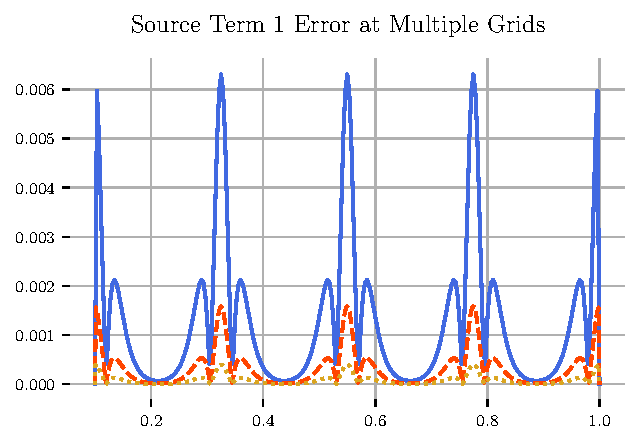
\includegraphics{/home/jeff-severino/SWIRL/CodeRun/04-plotReport/tex-outputs/SourceTermError1.pdf}
    \caption{LEE Source Term Error}
    \label{fig:7}
\end{figure}


\begin{figure}[!]
    \centering
    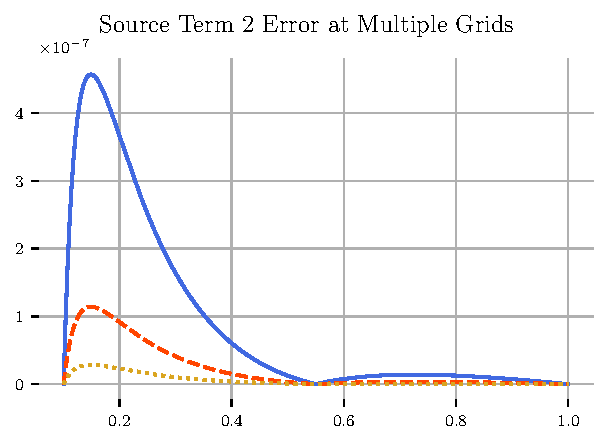
\includegraphics{/home/jeff-severino/SWIRL/CodeRun/04-plotReport/tex-outputs/SourceTermError2.pdf}
    \caption{LEE Source Term Error}
    \label{fig:7}
\end{figure}


\begin{figure}[!]
    \centering
    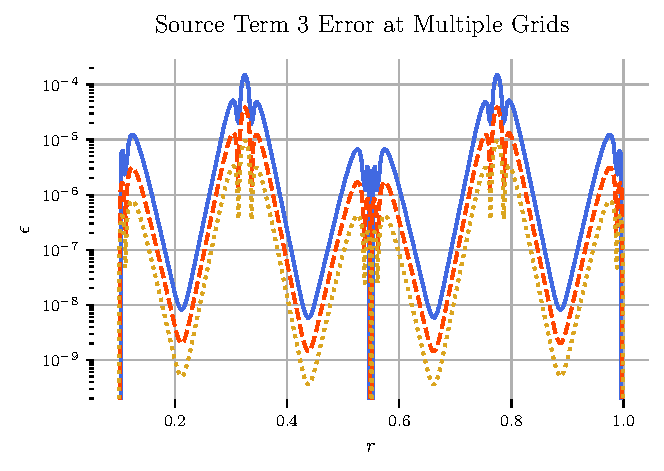
\includegraphics{/home/jeff-severino/SWIRL/CodeRun/04-plotReport/tex-outputs/SourceTermError3.pdf}
    \caption{LEE Source Term Error}
    \label{fig:7}
\end{figure}


\begin{figure}[!]
    \centering
    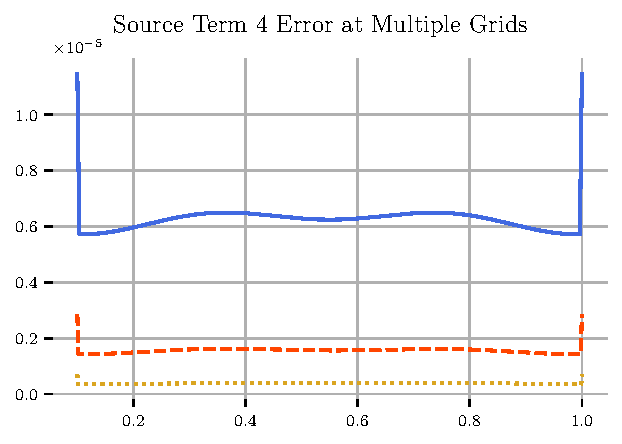
\includegraphics{/home/jeff-severino/SWIRL/CodeRun/04-plotReport/tex-outputs/SourceTermError4.pdf}
    \caption{LEE Source Term Error}
    \label{fig:7}
\end{figure}

\begin{figure}[!]
    \centering
    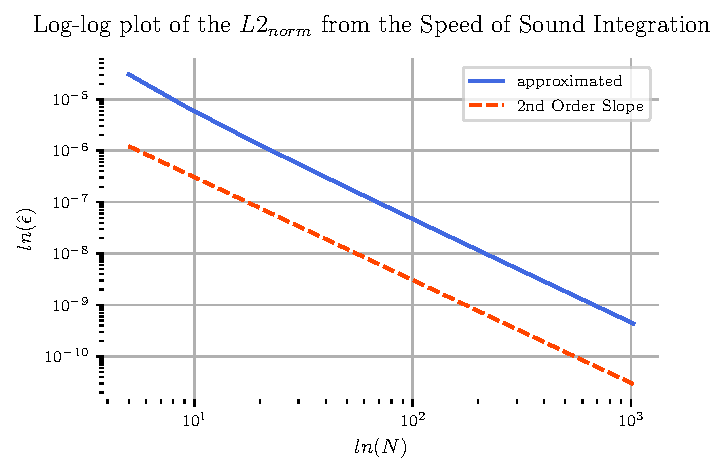
\includegraphics{/home/jeff-severino/SWIRL/CodeRun/04-plotReport/tex-outputs/SND_L2.pdf}
    \caption{L2 Norm comparison for the speed of sound integration for the compound trapezoidal rule}
    \label{fig:8}
\end{figure}



\begin{figure}[!]
    \centering
    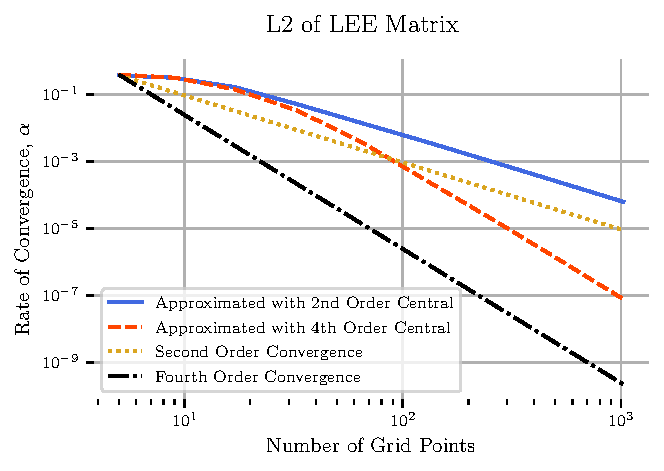
\includegraphics{/home/jeff-severino/SWIRL/CodeRun/04-plotReport/tex-outputs/LEE_L2.pdf}
    \caption{ROC  for the speed of sound integration for the compound trapezoidal rule}
    \label{fig:9}
\end{figure}


\begin{figure}[!]
    \centering
        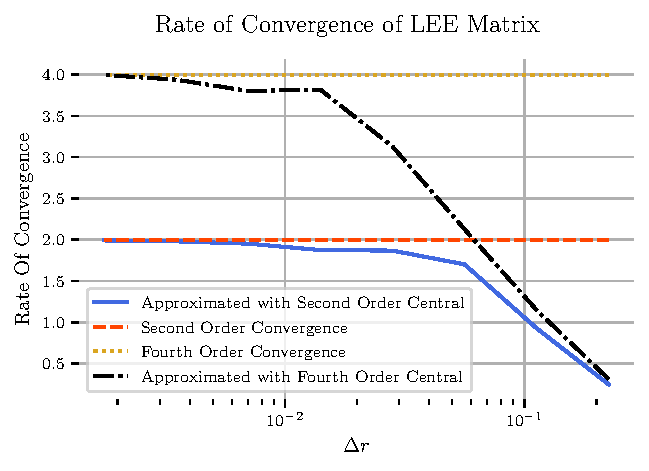
\includegraphics{/home/jeff-severino/SWIRL/CodeRun/04-plotReport/tex-outputs/LEE_ROC.pdf}
       \caption{ROC for the LEE using second and fourth order central differencing
       for the radial derivative}
        \label{fig:10}
\end{figure}





%%\begin{itemize}
%%    \item Kousen's Test Cases
%%        \subitem Cylinder, Uniform Flow with Liner (Table 4.3)
%%        \begin{align*}
%%            m &= 2 \\
%%            k &= \frac{\omega r_T}{A_T} = -1 \\
%%            M_x &= 0.5 \\
%%            \eta_T &= 0.72 + 0.42i\\
%%            \text{Confirm if 32 grid points is enough}
%%        \end{align*} 
%%        \subitem Cylinder, Shear Flow without Liner (Table 4.4)
%%        \begin{align*}
%%            m &= 0 \\
%%            kb &= \left(\frac{\omega r_T}{A_T}\right)b = 20 \\
%%            b &= r_{max} - r_{min} \\
%%            \tilde{r} = \frac{r}{b} \\
%%            M_x &= 0.3(1-\tilde{r})^{\frac{1}{7}} \\
%%            \eta_T &= 0\\
%%            \text{Confirm if 32 grid points is enough}
%%        \end{align*}
%%        \subitem Annulus, Shear Flow without Liner (Table 4.5)
%%        \begin{align*}
%%            m &= 0 \\
%%            kb &= \left(\frac{\omega r_T}{A_T}\right)b = 10 \\
%%            b &= r_{max} - r_{min}  = \frac{1}{7}\\
%%            k &= 70 \\
%%            \tilde{r} = \frac{r}{b} = 6.0 \\
%%            M_x &= 0.3\left(1 - 2 \left| \frac{r_{max}-r}{b} + 0.5 \right|  \right)^{\frac{1}{7}} \\
%%            \eta_T &= 0\\
%%            \text{Confirm if 32 grid points is enough}
%%        \end{align*}
%%        \subitem Annulus, Shear Flow with Liner (Table 4.6)
%%        \begin{align*}
%%            m &= 0 \\
%%            kb &= \left(\frac{\omega r_T}{A_T}\right)b = 10 \\
%%            b &= r_{max} - r_{min}  = \frac{1}{3}\\
%%            k &= 30 \\
%%            \tilde{r} = \frac{r}{b} = 2.0 \\
%%            M_x &= 0.3\left(1 - 2 \left| \frac{r_{max}-r}{b} + 0.5 \right|  \right)^{\frac{1}{7}} \\
%%            \eta_T &= 0.3 + 0.1i\\
%%            \text{Confirm if 32 grid points is enough}
%%        \end{align*}
%%\end{itemize}
\subsubsection{Test Case 1}
A comparison was conducted for a hollow cylinder undergoing uniform flow with
acoustic liners along the outer duct perimeter. The azimuthal mode number, reduced 
frequency, mach number and duct liner admittance is reported below,
\begin{align*}
    m &= 2 \\
    k &= \frac{\omega r_T}{A_T} = -1 \\
    M_x &= 0.5 \\
    \eta_T &= 0.72 + 0.42i
\end{align*} 
\begin{figure}[h!]
    \centering
    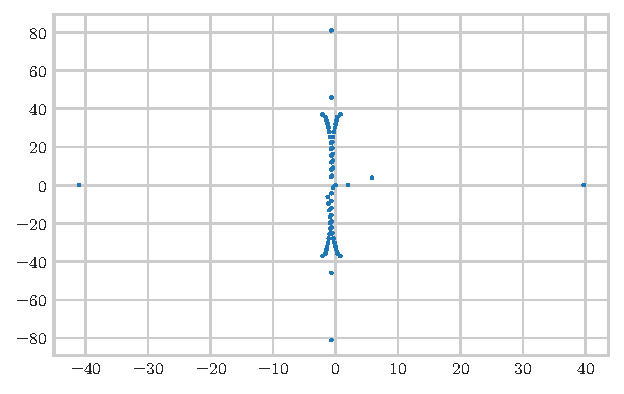
\includegraphics[width=\textwidth]{Chapter-5-Results/tex-outputs/gam.acc.scatter.Table4.3.pdf}
\end{figure}

\begin{figure}[h!]
    \centering
    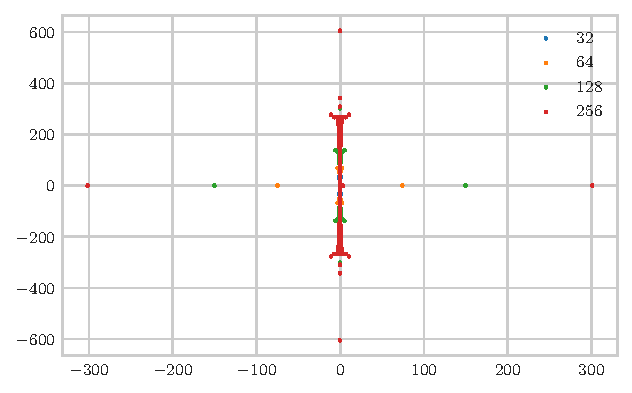
\includegraphics[width=\textwidth]{/home/jeff-severino/SWIRL/CodeRun/04-plotReport/tex-outputs/gam.nonconv.scatter_2nd_ord_comp.pdf}
\end{figure}

\begin{figure}[h!]
    \centering
    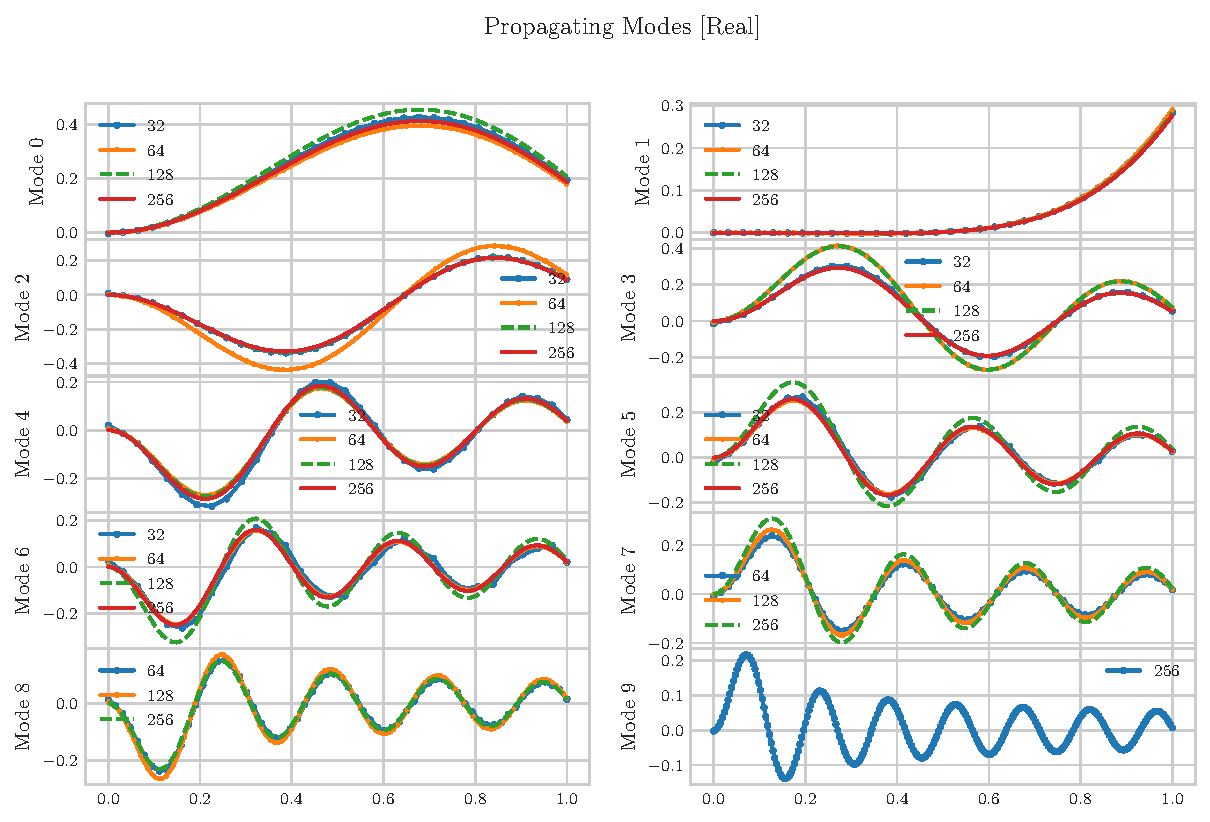
\includegraphics[width=\textwidth]{/home/jeff-severino/SWIRL/CodeRun/04-plotReport/tex-outputs/egv_prop_re.pdf}
    \label{fig:prop_re}
\end{figure}

\begin{figure}[h!]
    \centering
    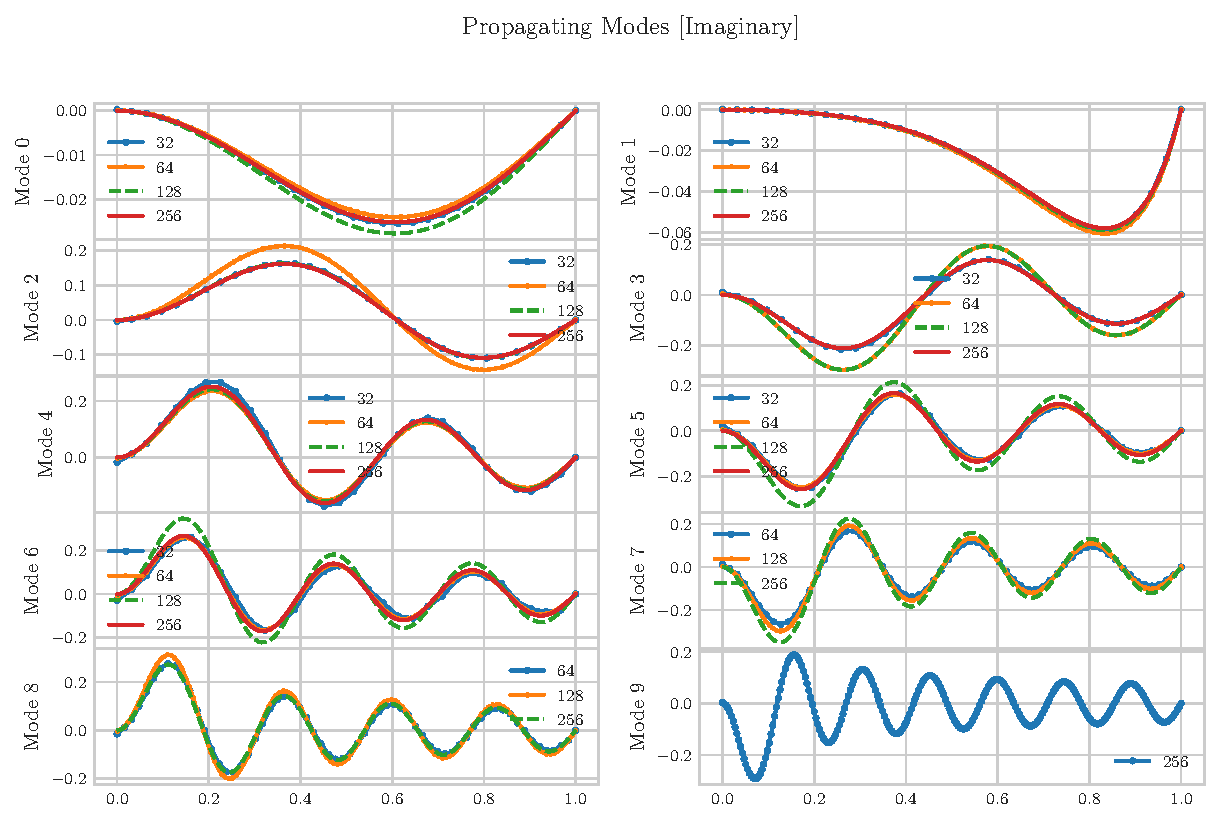
\includegraphics[width=\textwidth]{/home/jeff-severino/SWIRL/CodeRun/04-plotReport/tex-outputs/egv_prop_im.pdf}
    \label{fig:prop_im}
\end{figure}

\begin{figure}[h!]
    \centering
    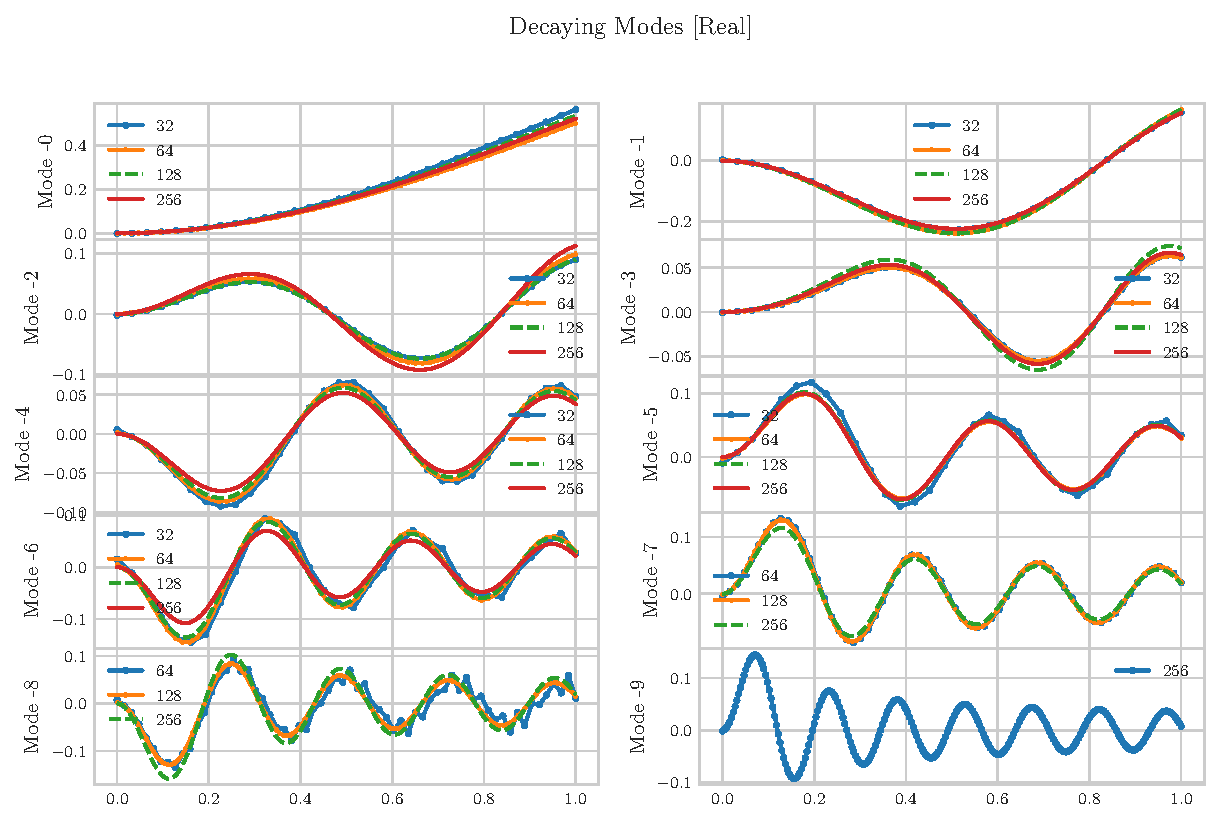
\includegraphics[width=\textwidth]{/home/jeff-severino/SWIRL/CodeRun/04-plotReport/tex-outputs/egv_decay_re.pdf}
    \label{fig:decay_re} 
\end{figure}

\begin{figure}[h!]
    \centering
    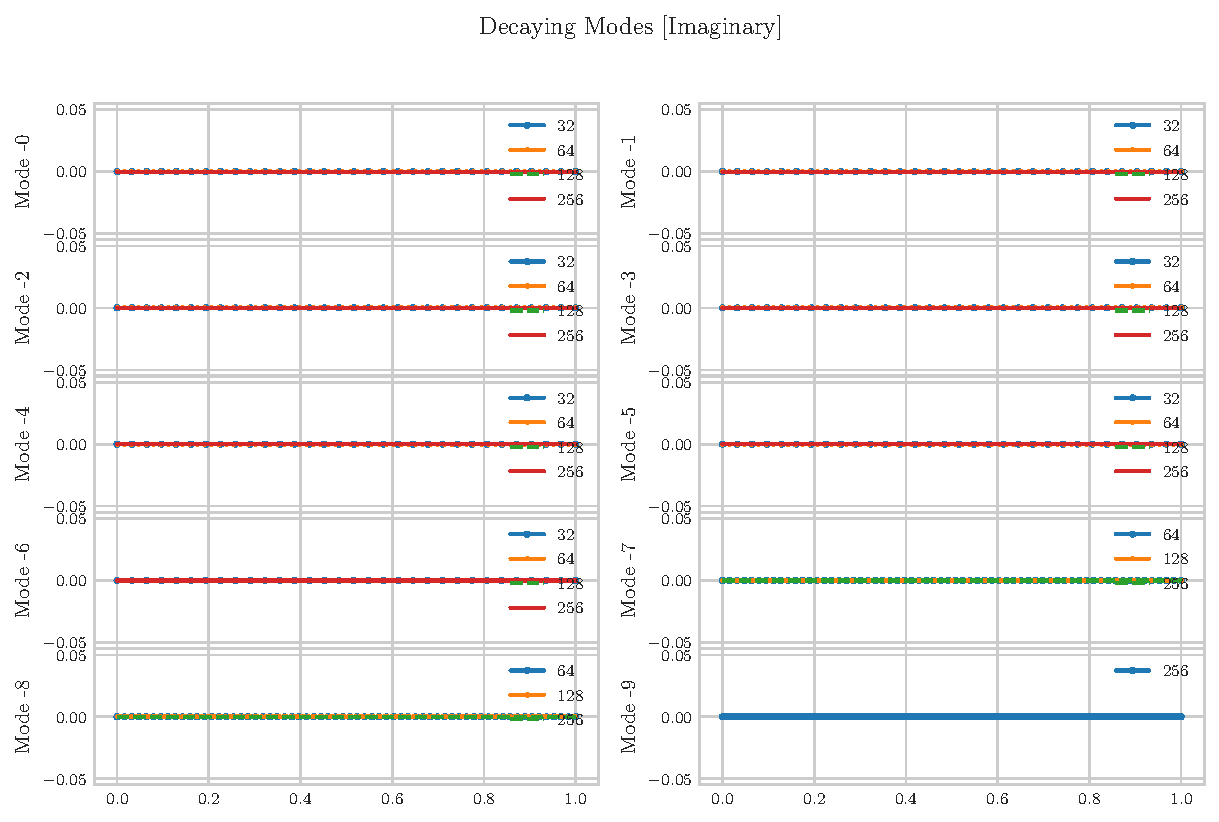
\includegraphics[width=\textwidth]{/home/jeff-severino/SWIRL/CodeRun/04-plotReport/tex-outputs/egv_decay_im.pdf}
    \label{fig:decay_im} 
\end{figure}








The results shown in \ref{Table43} are in moderately good agreement. The 
results were obtained by visually comparing the output in \verb|gam.acc| for 32 
grid points. Note that the indicies for the SWIRL deliverable are different that 
the ones obtained for the most recent version of the code. While the 
convective axial wavenumbers show agreement to machine precision, this is not 
particularly insightful given that there are an infinite number of possible solutions 
that could satisfy the eigenvalue problem. The results that are of concern 
are propagating modes that are not convecting with the mean flow.  The scatter plot
of the axial wavenumbers show some sporadic behaviour around the imaginary axis.
The results from the MMS along with this plot indicate that more grid points are going 
to be needed if a finite difference technique is to be used.

The first 10 propagating and decaying modes are plotted in \ref{fig:prop_re}-\ref{fig:decay_im}.



% It should be 
% noted that a spectral differencing method were using for Kousen's report and for
% srcF2008. 
%Using a higher order scheme would also improve accuracy.


\begin{table}
 \centering
 \begin{adjustbox}{width=1\textwidth}
     \small
 \begin{tabular}{c | r | r | r | r | r | r}
 \hline
 $\gamma^{\pm}_n$ & Kousen Ref. [15] & Kousen report & srcF2008 & index  & current & index\\
 \hline
 $\gamma_0^{+}$ & $ 0.620 - 5.014  i $ & $ 0.6195 - 5.0139 i$ & $ 0.61954  - 5.01386 i$ & 60  & 0.620755853112 - 5.00592416941i& 34 \\
 $\gamma_1^{+}$ & $-5.820 - 3.897  i $ & $-5.8195 - 3.8968 i$ & $-5.81953  - 3.89677 i$ & 58  &-0.581267772517 - 3.90050864568i& 33 \\
 $\gamma_2^{+}$ & $ 0.445 - 9.187  i $ & $ 0.4453 - 9.1868 i$ & $ 0.44533  - 9.18684 i$ & 59  &0.451569491142 -  9.12191317214i & 31 \\
 $\gamma_3^{+}$ & $ 0.453 - 13.062 i $ & $ 0.4539 - 13.062 i$ & $ 0.45389  - 13.0615 i$ & 57  &0.464247902898 - 12.8487472519i & 29 \\ 
 $\gamma_4^{+}$ & $ 0.480 - 16.822 i $ & $ 0.4795 - 16.822 i$ & $ 0.47952  - 16.8216 i$ & 55  &0.492340380223 - 16.3292825150i & 27 \\
 $\gamma_5^{+}$ & $ 0.503 - 20.531 i $ & $ 0.5029 - 20.531 i$ & $ 0.50287  - 20.5307 i$ & 51  &0.514522630594 -19.5817182568i& 25 \\
 $\gamma_6^{+}$ & $ 0.522 - 24.213 i $ & $ 0.5220 - 24.213 i$ & $ 0.52202  - 24.2129 i$ & 50  &0.516658239854 -22.5715880605i& 23 \\
 $\gamma_7^{+}$ & $ 0.538 - 27.880 i $ & $ 0.5376 - 27.880 i$ & $ 0.53754  - 27.8800 i$ & 48  & - & - \\
 $\gamma_8^{+}$ & $ 0.550 - 31.537 i $ & $ 0.5502 - 31.537 i$ & $ 0.55024  - 31.5368 i$ & 47  & - & - \\
 $\gamma_9^{+}$ & $ 0.589 - 49.75  i $ & $ 0.5891 - 49.754 i$ & $ 0.58745  - 49.7669 i$ & 33  &- &- \\ \hline
 $\gamma_0^{-}$ & $ 0.410 + 1.290  i $ & $ 0.4101 + 1.2904 i$ & $ 0.41009  + 1.29037 i$ & 64  &0.409973310292  + 1.29020083859i& 64 \\
 $\gamma_1^{-}$ & $ 1.259 + 6.085  i $ & $ 1.2595 + 6.0852 i$ & $ 1.25949  + 6.08517 i$ & 63  &1.25530612217  + 6.07214375548i & 62 \\
 $\gamma_2^{-}$ & $ 1.146 + 9.668  i $ & $ 1.1457 + 9.6679 i$ & $ 1.14567  + 9.66787 i$ & 62  &1.13696444935  + 9.59622801724i &  60\\
$\gamma_3^{-}$ & $ 1.022 + 13.315 i $ & $ 1.0218 + 13.315 i$ & $ 1.02183  + 13.3150 i$ & 61  &1.00950576515 + 13.0957277529i & 58  \\
 $\gamma_4^{-}$ & $ 0.943 + 16.977 i $ & $ 0.9425 + 16.977 i$ & $ 0.94250  + 16.9767 i$ & 56  &0.928059983039 +  16.4791343118i& 56  \\
 $\gamma_5^{-}$ & $ 0.891 + 20.635 i $ & $ 0.8908 + 20.635 i$ & $ 0.89075  + 20.6353 i$ & 54  &0.856678172769 +  22.6544943903i & 52 \\
 $\gamma_6^{-}$ & $ 0.855 + 24.288 i $ & $ 0.8549 + 24.288 i$ & $ 0.85490  + 24.2883 i$ & 53  &0.941762848775 +  25.3460188358i & 50 \\
 $\gamma_7^{-}$ & $ 0.829 + 27.937 i $ & $ 0.8288 + 27.937 i$ & $ 0.82877  + 27.9369 i$ & 52  &- & - \\
 $\gamma_8^{-}$ & $ 0.809 + 31.581 i $ & $ 0.8089 + 31.581 i$ & $ 0.80891  + 31.5812 i$ & 49  &- & - \\
 $\gamma_9^{-}$ & $ 0.755 + 49.77  i $ & $ 0.7547 + 49.772 i$ & $ 0.75658  + 49.7851 i$ & 39  &- & - \\ \hline
 \end{tabular}
\end{adjustbox}
 \caption{Table 4.3 data}
 \label{Table43}
\end{table}

